\documentclass[11pt,a4paper]{report}
\usepackage[document]{ragged2e}
\usepackage{setspace}
\usepackage[utf8]{inputenc}
\usepackage{amsmath}
\usepackage{amsfonts}
\usepackage{amssymb}
\usepackage{textcomp}
\usepackage{gensymb}
\usepackage{graphicx}
\graphicspath{ {~/LatexFiles/TrabajoPracticoADC} }
\author{Marcos Rolando}
\begin{document}
\spacing{1.25}

\section*{Análisis general de la función de transferencia}

\subsection*{Tipo de filtro}

Dada la función de transferencia asignada
\[H(s)=\frac{3948 \cdot s^2}{s^4+88,86 \cdot s^3+7,935 \cdot 10^5 \cdot s^2+3,508 \cdot 10^7 \cdot s+1,559 \cdot 10^{11}}\]
procederemos a analizar su comportamiento en $s=0$ y $s\longrightarrow\infty$.

\bigskip
En primer lugar analizamos el caso $s=0$ para el cual tenemos que 
\[H(0) = \frac{3948 \cdot 0^2}{0^4+88,86 \cdot 0^3+7,935 \cdot 10^5 \cdot 0^2+3,508 \cdot 10^7 \cdot 0+1,559 \cdot 10^{11}}\]

obteniendo entonces que
\[H(0) = 0\]

Analizando ahora el caso $s\longrightarrow\infty$ tenemos que
\[\lim_{s \to \infty} H(s) = 0\]
dado que el grado del denominador es dos veces mayor al del numerador.

\bigskip
En base a los valores obtenidos podemos entonces afirmar que se trata de un
filtro pasabanda dado que la transferencia es nula para frecuencias bajas y altas.

\subsection*{Ceros y polos}

En principio, es trivial ver que el único cero de la función $H(s)$ es
$s = 0$ y dado que está elevado al cuadrado se deduce que el cero es doble.

\bigskip
Por otro lado tenemos los polos, cuyo cálculo no es trivial. Dado que el denominador de la función es de grado cuatro tendremos entonces cuatro raíces. Debido a esto
y a que los coeficientes del polinomio complejizan el desarrollo del cálculo de 
dichas raíces, se calcularán entonces mediante calculadora. 

\bigskip
Obtenemos que
\[p_{1,2} \approx -21,40 \pm 606,9j\]
\[p_{3,4} \approx -23,03 \pm 649,8j\]
donde $p_{1,2}$ y $p_{3,4}$ son los pares conjuados que componen los cuatros
polos de $H(s)$, y donde el primer subíndice corresponde al conjugado cuya parte imaginaria es positiva mientras que el segundo subíndice corresponde al de parte imaginaria negativa.

\subsection*{Cálculo de $W_{0}$ y Q}

Dado que el denominador se compone de dos pares de raíces complejas conjugadas tendrá entonces un $W_{0}$ y Q para cada par. Para obtenerlos debemos primero reescribir la función $H(s)$ a la forma
\[H(s)=\frac{3948 \cdot s^2}{(a \cdot s^2+b \cdot s+c) \cdot (d \cdot s^2+e \cdot s+f)}\]
donde las letras corresponden a valores que debemos calcular de forma tal que dicha
ecuación sea equivalente a la fórmula original de $H(s)$.

\bigskip
Para conseguir esto es conveniente utilizar las raíces del denominador de $H(s)$ (los polos de la función) expresando la función como
\[H(s)=\frac{3948 \cdot s^2}{k \cdot (s-p_{1}) \cdot (s-p_{2}) \cdot (s-p_{3}) \cdot (s-p_{4})}\]
donde k es el factor del término $k*s^4$ y, para nuestra función en particular,
se da que $k=1$. 

\bigskip
Luego, multiplicando los polos conjuados entre sí obtenemos
\[H(s)=\frac{3948 \cdot s^2}{(s^2-(p1+p2) \cdot s+p_{1} \cdot p_{2}) \cdot (s^2-(p3+p4) \cdot s+p_{3} \cdot p_{4})}\]

\bigskip
Sean $z_{1}$ y $z_{2}$ dos números complejos conjugados tenemos que 

\[z1+z2=2\Re(z_{1}) = 2\Re(z_{2})\] 
\[z1 \cdot z2=|z_{1}|^2=|z_{2}|^2\] 

Aplicando estas propiedades a $p_{1,2}$ y 
$p_{3,4}$ obtenemos la expresión
\[H(s)=\frac{3948 \cdot s^2}{(s^2-2\Re(p1) \cdot s+|p_{1}|^2) \cdot (s^2-2\Re(p3) \cdot s+|p_{3}|^2)}\]

\bigskip
$W_{0}$ y Q vienen dados por $s^2+\frac{W_{0}}{Q} \cdot s + W_{0}^2$. Ejemplificando para el primer factor del denominador tendríamos entonces que 
\[W_{0_{1}} = |p1|\]
\[Q_{1} = -\frac{W_{0_{1}}}{2\Re(p_{1})}\]

\bigskip
Reemplazando obtenemos finalmente que
\[W_{0_{1}} \approx 607,3 \frac{r}{s}\]
\[Q_{1} \approx 14,19\]
\[W_{0_{2}} \approx 650,2 \frac{r}{s}\]
\[Q_{2} \approx 14,12\]
siendo $W_{0_{1}}$ y $Q_{1}$ los valores correspondientes al polinomio de segundo 
grado cuyas raíces son $p_{1,2}$ y $W_{0_{2}}$ y $Q_{2}$ los correspondientes
al polinomio de segundo grado de raíces $p_{3,4}$.

\bigskip
Finalmente, reemplazando con los valores de W y Q obtenidos podemos expresar la función de transferencia como
\[H(s) \approx \frac{3948 \cdot s^2}{(s^2+42,81 \cdot s +368,8 \cdot 10^3)
\cdot (s^2+46,05 \cdot s + 422,8 \cdot 10^3)}\]

\subsection*{Diagramas de Bode}

A continuación se presentan los diagramas de Bode tanto de módulo como de fase (en grados sexagesimales) de la función $H(s)$ junto con una breve descripción explicando
lo obtenido. Para los diagramas de Bode se analiza el caso $s=jw$ donde $w$ se mide
en $\frac{r}{s}$ (radianes por segundo).

\begin{figure}[h!]
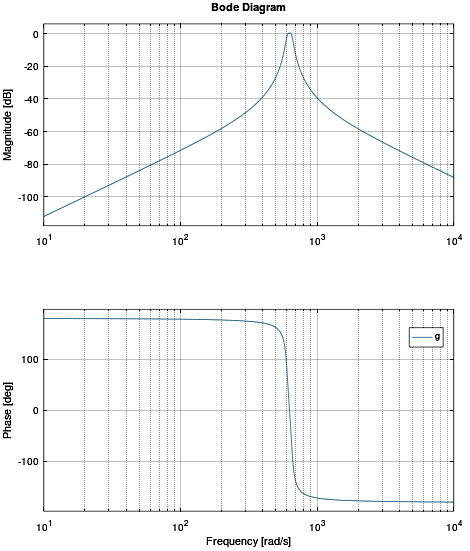
\includegraphics[scale=0.7]{DiagramasBode.png}
\caption{Diagramas de Bode}
\end{figure}

\newpage
En primer lugar tenemos el diagrama de módulo de Bode, es decir, el módulo de 
$H(jw)$ medido en dB (decibeles) el cual viene dado por la\\ fórmula
\[20 \cdot \log(|H(jw)|) dB\]
Dado que el filtro es un pasabanda era lo esperable
observar que para frecuencias bajas ($w\longrightarrow0$) y altas ($w\longrightarrow\infty$) el gráfico tendiera a $-\infty$ dado que este tipo de
filtro se caracteriza por anular la función de transferencia para dichas frecuencias.
Esto puede verse matemáticamente en base al análisis previo realizado donde se calculó que $H(0) = 0$ y $\lim_{s \to \infty} H(s) = 0$, luego 
$\lim_{x \to 0} \log(x) = -\infty$ lo cual explica lo observado en el primer gráfico.

\bigskip
El segundo gráfico es el diagrama de fase de Bode (en grados sexagesimales). 
Los valores de este gráfico vienen dados por la fórmula 
\[\arctan(\frac{\Im(H(jw))}{\Re(H(jw)})\]
Dado que el numerador de la función se compone de un único término $3948 \cdot s^2$ 
tenemos que la constante positiva aporta $0\degree$ mientras que el $s^2$ aporta
$180\degree$ (recordemos que $s=jw$ lo cual tiene un ángulo de $90\degree$, luego elevar al cuadrado duplica el ángulo y obtenemos $180\degree$).

\bigskip
Al acercarnos a las frecuencias $W_{0}$ de los polos vemos como empieza a disminuir el ángulo a un ritmo de $-180 \frac{grad}{dec}$ aproximadamente. En rigor, en principio hay un intervalo donde disminuye $-90 \frac{grad}{dec}$ pero dicho intervalo no es apreciable dada la escala y cercanía entre los $W_{0}$. 
Finalmente, una vez alcanzado el valor $W=10 \cdot W_{0}$ los polos ya no aportan
pendiente decreciente y se estabiliza el gráfico nuevamente, quedando en este caso
en $-180\degree$ aproximadamente.

\newpage
\section*{Respuesta gráfica del sistema a distintas señales}

A continuación se presentan gráficos de respuestas del sistema a distintos tipos
de señales y frecuencias.

\subsubsection*{Respuesta al escalón}

\begin{figure}[h!]
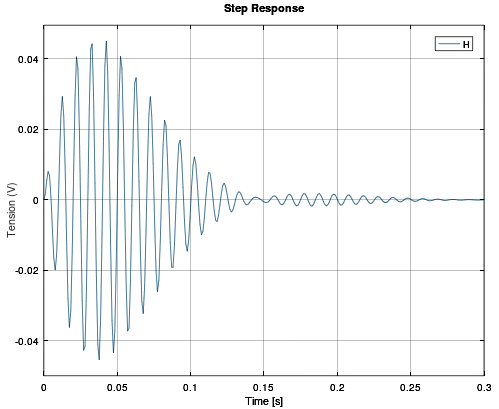
\includegraphics[scale=0.7]{RtaEscalon.png}
\caption{Respuesta al escalón}
\end{figure}

\newpage
\begin{figure}[h!]
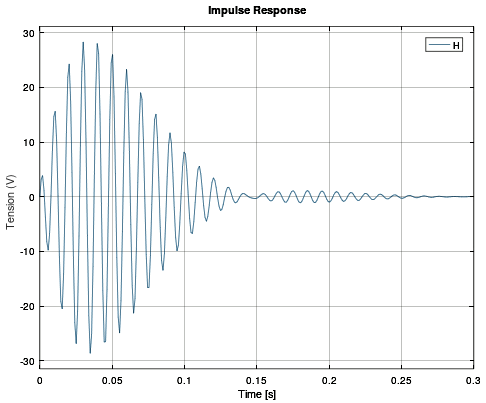
\includegraphics[scale=0.7]{RtaImpulso.png}
\caption{Respuesta al impulso}
\end{figure}


\end{document}